This project was written as a semester project by group SW805F14 - Software students from the Department of Computer Science at Aalborg University in the Spring of 2014. The report documents the implementation of the Dishcover application. The application is developed for the Android platform. The reader is expected to be familiar with Java, UML, and the Android platform. We have included our knowledge from all our previous semesters.
\\\\
Database access:\\\\
URL: \textbf{http://figz.dk/phpmyadmin}\\
Username: \textbf{sw8}\\
Password: \textbf{sw8}\\\\
When reading the report, there are a few things the reader should be aware of:
\begin{itemize}
\item When a reference to a source of a section or paragraph is given, the number of the source is written inside square brackets $[\;]$. The number is a reference to the bibliography list on page \pageref{chap:bib}.
\item When "we/us/our" is mentioned in the report, it is a referral to the authors of the report
\item Throughout the report three different terms are used: Activity, Fragment, and Page. These are used to describe different kind of user interfaces in Android. ``Page'' is used in contexts where it is not relevant whether it is an activity or a fragment
\begin{description}
\item[Activity] An activity is a single focused thing that the user can do. You can also say that it is a window which is either full-screen or floating. \citep{activity}
\item[Fragment] A fragment inherits from activity and thus has its own lifecycle. Fragments are nested in activities, and can be used to build a multi-pane user interface. \citep{fragment}
\end{description}
\item In class diagrams a minus symbol denotes a private attribute/method, a plus symbol denotes a public attribute/method, and a sharp symbol denotes a protected attribute/method. Italic class names are abstract classes.
\begin{center}
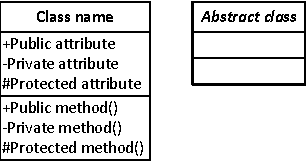
\includegraphics[width=0.35\linewidth]{img/umltheory.pdf}
\end{center}
\end{itemize}

We would like to thank our supervisor Ramin Sadre for the feedback he has given throughout the project.